\documentclass[pdflatex,compress,mathserif]{beamer}

%\usetheme[dark,framenumber,totalframenumber]{ElektroITK}
\usetheme[darktitle,framenumber,totalframenumber]{ElektroITK}

\usepackage{amsmath}
\usepackage{mathtools}
\usepackage{graphicx}
\usepackage{multicol}
\usepackage[bahasai]{babel}

\newcommand*{\Scale}[2][4]{\scalebox{#1}{$#2$}}%

\title{METODE NUMERIK}
\subtitle{Solusi Sistem Persamaan Lanjar}

\author{Tim Dosen Pengampu}

\begin{document}
	
\maketitle

\section{Pengantar}

\begin{frame}
	\frametitle{Pengantar}
	\begin{itemize}
		\item \textbf{Persoalan:} Temukan vektor $ x $ yang memenuhi sistem persamaan lanjar \[ Ax = b \] yang dalam hal ini,
		\begin{align*}
			A &= [a_{ij}] \text{ adalah matriks berukuran } n \times n\\
			x &= [x_{j}]  \text{ adalah matriks berukuran } n \times 1 \\
			b &= [b_{j}]  \text{ adalah matriks berukuran } n \times 1 \text{ (vektor kolom) }
		\end{align*}
	\end{itemize}
	\[\Scale[0.7]{
		\begin{matrix}
			a_{11}x_1 + a_{12}x_2 + \dots + a_{1n}x_n &= b_1 \\
			a_{21}x_1 + a_{22}x_2 + \dots + a_{2n}x_n &= b_2 \\
			&\vdots\\
			a_{n1}x_1 + a_{n2}x_2 + \dots + a_{nn}x_n &= b_n
		\end{matrix}
		\rightarrow
		\begin{bmatrix}
			a_{11} & a_{12} & a_{13} & \dots & a_{1n} \\
			a_{21} & a_{22} & a_{23} & \dots & a_{2n} \\
			a_{31} & a_{32} & a_{33} & \dots & a_{3n} \\
			& & & \vdots &  \\
			a_{n1} & a_{n2} & a_{n3} & \dots & a_{nn}
		\end{bmatrix}
		\begin{bmatrix}
			x_1 \\
			x_2 \\
			x_3 \\
			\vdots\\
			x_n \\
		\end{bmatrix}
		=
		\begin{bmatrix}
			b_1 \\
			b_2 \\
			b_3 \\
			\vdots\\
			b_n \\
		\end{bmatrix}
	}\]
\end{frame}

\begin{frame}
	\frametitle{Metode-Metode Penyelesaian}
	\begin{itemize}
		\item Metode penyelesaian praktis sistem persamaan lanjar yang dibahas di sini adalah:
		\begin{enumerate}
			\item Metode eliminasi Gauss 
			\item Metode eliminasi Gauss-Jordan
			\item Metode matriks balikan
			\item Metode dekomposisi LU
			\item Metode lelaran Jacobi
			\item Metode lelaran Gauss-Seidel.
		\end{enumerate}
		\item Metode 2, 3, dan 4, didasarkan pada Metode 1
		\item Metode 5 dan 6 dikembangkan dari gagasan metode lelaran pada solusi persamaan nirlanjar
	\end{itemize}
\end{frame}

\section{Metode Eliminasi Gauss}

\begin{frame}
	\frametitle{Metode Eliminasi Gauss}
	\begin{itemize}
		\item Metode ini berangkat dari kenyataan bahwa bila matriks $ A $ berbentuk segitiga atas seperti sistem persamaan berikut ini
		\begin{equation*}
			\begin{bmatrix}
				a_{11} & a_{12} & a_{13} & \cdots & a_{1n}\\
				0 & a_{22} & a_{23} & \cdots & a_{2n}\\
				0 & 0 & a_{33} & \cdots & a_{3n}\\
				& & & \vdots & \\
				0 & 0 & 0 & \cdots & a_{nn}\\
			\end{bmatrix}
			\begin{bmatrix}
			x_1\\
			x_2\\
			x_3\\
			\vdots\\
			x_n\\
			\end{bmatrix}
			=
			\begin{bmatrix}
			b_1\\
			b_2\\
			b_3\\
			\vdots\\
			b_n\\
			\end{bmatrix}
		\end{equation*}
		\item maka solusinya dapat dihitung dengan \textbf{teknik penyulihan
		mundur} (\textit{backward substitution})
	\end{itemize}
\end{frame}

\begin{frame}
	\scalebox{0.7}{\parbox{.5\linewidth}{%
	\begin{align*}
		a_{nn}x_n = b_n &\rightarrow x_n = b_n / a_{nn} \\
		a_{n-1,n-1}x_{n-1} + a_{n-1,n}x_{n} = b_{n-1} &\rightarrow x_{n-1} = \frac{b_{n-1} - a_{n-1,n}x_n}{a_{n-1,n-1}}\\
		a_{n-2,n-2}x_{n-2} + a_{n-2,n-1}x_{n-1} + a_{n-2,n}x_{n} = b_{n-2} &\rightarrow x_{n-2} = \frac{b_{n-2} - a_{n-2,n-1}x_{n-1} - a_{n-2,n}x_{n}}{a_{n-2,n-2}}\\
	\end{align*}
	}}
	\begin{itemize}
		\item Sekali $ x_n $, $ x_{n-1} $, $ x_{n-2} $, $\dots$, $ x_{k+1} $ diketahui, maka nilai $ x_k $ dapat dihitung dengan
		\[ x_k = \frac{b_k - \sum_{j=k+1}^{n}a_{kj}x_j}{a_{kk}}.\qquad k=n-1, n-2, \dots, 1 \text{ dan } a_{kk} \neq 0 \]
	\end{itemize}
\end{frame}

\begin{frame}
	\frametitle{Contoh 1}
	\begin{itemize}
		\item Selesaikan sistem persamaan lanjar berikut dengan teknik penyulihan mundur
		\begin{align*}
			4x_1 - x_2 + 2x_3 + 3x_4 &= 20 \\
			-2x_2 + 7x_3 - 4x_4 &= -7 \\
			6x_3 + 5x_4 &= 4 \\
			3x_4 &= 6
		\end{align*}
	\end{itemize}
\end{frame}

\begin{frame}
	\begin{itemize}
		\item Penyelesaian:
		\begin{align*}
		x_4 &= 6/3 = 2 \\
		x_3 &= \frac{(4-5(2))}{6} = -1 \\
		x_2 &= \frac{-7-7(-1)+4(2)}{-2} = -4 \\
		x_1 &= \frac{20 + 1(-4) - 2(-1)-3(2)}{4} = 3
		\end{align*}
		\item Jadi, solusinya adalah \[ x = \begin{bmatrix}
			3 \\ -4 \\ -1 \\ 2
		\end{bmatrix} \]
	\end{itemize}
\end{frame}

\begin{frame}
	\begin{itemize}
		\item Metode eliminasi Gauss pada prinsipnya bertujuan mentransformasi sistem $ Ax = b $ menjadi sistem \[ Ux = y \] dengan $ U $ adalah \textbf{matriks segitiga atas}.
		\item Selanjutnya solusi $ x $ dapat dihitung dengan \textbf{teknik penyulihan mundur}.
	\end{itemize}
\end{frame}

\begin{frame}
	\begin{align*}
	[A,b]
	&\rightarrow
	[U,y]
	\\
	\left[
	\begin{matrix}
	a_{11} & a_{12} & a_{13} & a_{14}\\
	a_{21} & a_{22} & a_{23} & a_{24}\\
	a_{31} & a_{32} & a_{33} & a_{34}\\
	a_{41} & a_{42} & a_{43} & a_{44}
	\end{matrix}
	\right|
	\left.
	\begin{matrix}
	b_{1}\\
	b_{2}\\
	b_{3}\\
	b_{4}
	\end{matrix}
	\right]
	&\rightarrow
	\left[
	\begin{matrix}
	a_{11} & a_{12} & a_{13} & a_{14}\\
	0 & a_{22}^{(1)} & a_{23}^{(1)} & a_{24}^{(1)}\\
	0 & 0 & a_{33}^{(2)} & a_{34}^{(2)}\\
	0 & 0 & 0 & a_{44}^{(3)}
	\end{matrix}
	\right|
	\left.
	\begin{matrix}
	b_{1}\\
	b_{2}^{(1)}\\
	b_{3}^{(2)}\\
	b_{4}^{(3)}
	\end{matrix}
	\right]
	\end{align*}
\end{frame}

\begin{frame}
	Proses eliminasi terdiri atas tiga operasi baris elementer:
	\begin{enumerate}
		\item \textbf{Pertukaran:} Urutan dua persamaan dapat ditukar karena pertukaran tersebut tidak mempengaruhi solusi akhir.
		\item \textbf{Penskalaan:} Persamaan dapat dikali dengan konstanta bukan nol, karena perkalian tersebut tidak mempengaruhi solusi akhir.
		\item \textbf{Penggantian:} Persamaan dapat diganti dengan penjumlahan persamaan itu dengan gandaan persamaan lain. Misalnya persamaan diganti dengan selisih persamaan itu dengan dua kali persamaan lain; yaitu
		\[ \text{baris}_r := \text{baris}_r - m_{p,r}\text{baris}_p \]
	\end{enumerate}
\end{frame}

\begin{frame}
	\begin{itemize}
		\item Nilai $ a_{r, r} $ pada posisi $ (r, r) $ yang digunakan untuk mengeliminasi $ x_r $ pada baris $ r + 1, r + 2, \dots, N $ dinamakan \textbf{elemen pivot} dan persamaan pada baris ke-$ r $ disebut \textbf{persamaan pivot}.
		\item Ada kemungkinan pivot bernilai nol sehingga pembagian dengan nol tidak dapat dielakkan.
		\item Tata-ancang eliminasi yang tidak mempedulikan nilai pivot adalah tatancang yang naif (naive) atau sederhana. Metode eliminasi Gauss seperti ini dinamakan \textbf{metode eliminasi Gauss naif} (\textit{naive Gaussian elimination}).
		\item Pada metode eliminasi Gauss naif tidak ada operasi pertukaran baris dalam rangka menghindari pivot yang bernilai nol itu.
	\end{itemize}
\end{frame}

\begin{frame}
	\frametitle{Contoh 2}
	\begin{itemize}
		\item \textbf{Persoalan:}  Selesaikan sistem persamaan lanjar dengan metode eliminasi Gauss naif:
		\begin{align*}
			2x_1 + 3x_2 - x_3 &= 5 \\
			4x_1 + 4x_2 - 3x_3 &= 3 \\
			-2x_1 + 3x_2 - x_3 &= 1
		\end{align*}
	\end{itemize}
\end{frame}

\begin{frame}
	\begin{itemize}
		\item \textbf{Penyelesaian:}
		\[
			\Scale[0.8]{
			\left[
				\begin{matrix}
				\textbf{2} & 3 & -1 \\
				4 & 4 & -3 \\
				-2 & 3 & -1
				\end{matrix}
			\right|
			\left.
				\begin{matrix}
				5 \\
				3 \\
				1
				\end{matrix}
			\right]
				\begin{matrix}
				\\
				R_2 - \frac{4}{2}R_1 \\
				R_3 - \frac{-2}{2}R_1
				\end{matrix}
			\left[
				\begin{matrix}
				2 & 3 & -1 \\
				0 & \textbf{-2} & -1 \\
				0 & 6 & -2
				\end{matrix}
			\right|
			\left.
				\begin{matrix}
				5 \\
				-7 \\
				6
				\end{matrix}
			\right]
				\begin{matrix}
				\\
				\\
				R_3 - \frac{6}{-2}R_1
				\end{matrix}
			\left[
				\begin{matrix}
				2 & 3 & -1 \\
				0 & -2 & -1 \\
				0 & 0 & -5
				\end{matrix}
			\right|
			\left.
				\begin{matrix}
				5 \\
				-7 \\
				-15
				\end{matrix}
			\right]}
		\]
		\item Solusi sistem diperoleh dengan teknik penyulihan mundur sebagai berikut:
		\begin{align*}
		-5x_3 = -15 &\rightarrow x_3 = 3 \\
		-2x_2 - x_3 = -7 &\rightarrow x_2 = (-7 + 3)/-2 = 2 \\
		2x_1 + 3x_2 - x_3 = 5 &\rightarrow x_1 = (5 + 3 - 6)/2 = 1
		\end{align*}
		\item Jadi, solusinya adalah $ x = (1,2,3)^T $
	\end{itemize}
\end{frame}

\begin{frame}
	\frametitle{Kelemahan eliminasi Gauss naif}
	\begin{itemize}
		\item Jika pivot $ a_{pp} = 0 $, baris ke-$ k $ tidak dapat digunakan untuk memgeliminasi elemen pada kolom $ p $, karena terjadinya pembagian dengan nol.
		\item Oleh karena itu, pivot yang bernilai nol harus dihindari dengan tata-ancang (\textit{strategy pivoting}).
	\end{itemize}
\end{frame}

\subsection{Tata-ancang Pivoting}

\begin{frame}
	\frametitle{Tata-ancang Pivoting}
	\begin{itemize}
		\item Jika $ a_{p,p}^{(p-1)} = 0 $, cari baris $ k $ dengan $ a_{k,p} \neq 0 $ dan $ k > p $, lalu pertukarkan baris $ p $ dan baris $ k $.
		\item Metode eliminasi Gauss dengan tata-ancang pivoting disebut metode eliminasi Gauss yang diperbaiki (\textit{modified Gaussian elimination}).
	\end{itemize}
\end{frame}

\begin{frame}
	\frametitle{Contoh 3}
	\begin{itemize}
		\item \textbf{Persoalan:} Selesaikan sistem persamaan lanjar berikut dengan metode eliminasi Gauss yang menerapkan tata-ancang pivoting.
		\begin{align*}
			x_1 + 2x_2 + x_3 &= 2 \\
			3x_1 + 6x_2 &= 9 \\
			2x_1 + 8x_2 + 4x_3 &= 6
		\end{align*}
	\end{itemize}
\end{frame}

\begin{frame}
	\begin{itemize}
		\item \textbf{Penyelesaian:}
	\end{itemize}
	
	\[
	\left[
		\begin{matrix}
			\textbf{1} & 2 & 1 \\
			3 & 6 & 0 \\
			2 & 8 & 4
		\end{matrix}
	\right|
	\left.
		\begin{matrix}
			2 \\
			9 \\
			6
		\end{matrix}
	\right]
	\begin{matrix}
		\\
		R_2 - \frac{3}{1}R_1 \\
		R_3 - \frac{2}{1}R_1
	\end{matrix}
	\left[
		\begin{matrix}
			1 & 2 & 1 \\
			0 & \textbf{0} & -3 \\
			0 & 4 & 2
		\end{matrix}
	\right|
	\left.
		\begin{matrix}
			2 \\
			3 \\
			2
		\end{matrix}
	\right]
	\begin{matrix}
	\\
	R_2 \Leftrightarrow R_3\\
	\end{matrix}
	\left[
	\begin{matrix}
	1 & 2 & 1 \\
	0 & 4 & 2 \\
	0 & 0 & -3
	\end{matrix}
	\right|
	\left.
	\begin{matrix}
	2 \\
	2 \\
	3
	\end{matrix}
	\right]
	\]
\end{frame}

\begin{frame}
	\frametitle{Pivoting Sederhana}
	\begin{itemize}
		\item Melakukan pertukarkan baris untuk menghindari \textit{pivot} yang bernilai nol adalah cara \textit{pivoting} yang sederhana (\textit{simple pivoting}).
		\item Masalah lain dapat juga timbul bila elemen \textit{pivot} sangat dekat ke nol, karena jika elemen \textit{pivot} sangat kecil dibandingkan terhadap elemen lainnya, maka galat pembulatan dapat muncul.
		\item Jadi, disamping menghindari pembagian dengan nol, tata-ancang \textit{pivoting} dapat juga diperluas untuk mengurangi galat pembulatan.
		\item Terdapat 2 macam \textit{pivoting} yaitu \textbf{\textit{pivoting} sebagian} dan \textbf{\textit{pivoting} lengkap}.
	\end{itemize}
\end{frame}

\begin{frame}
	\frametitle{Pivoting Sebagian (Partial Pivoting)}
	\begin{itemize}
		\item Pada tata-ancang \textit{pivoting} sebagian, \textit{pivot} dipilih dari semua elemen pada kolom $ p $ yang mempunyai nilai mutlak terbesar,
		\[ |a_{k,p}| = \text{max}\{|a_{p,p}|,|a_{p+1,p}|,\dots,|a_{n-1,p}|, |a_{n,p}|\} \]
		\item  lalu pertukarkan baris ke-$ k $ dengan baris ke-$ p $.
		\[
		\left[
		\begin{matrix}
			x & x & x & x \\
			0 & \textbf{x} & x & x \\
			0 & \textbf{x} & x & x \\
			0 & \textbf{x} & x & x \\
		\end{matrix}
		\right|
		\left.
		\begin{matrix}
		x \\ x \\ x \\ x
		\end{matrix}
		\right]
		\] cari $ |\textbf{x}| $ terbesar, lalu pertukarkan barisnya dengan baris ke-2
	\end{itemize}
\end{frame}

\begin{frame}
	\begin{itemize}
		\item Perhatikanlah bahwa teknik pivoting sebagian juga sekaligus menghindari pemilihan \textit{pivot} = 0 (sebagaimana pada \textit{simple pivoting})
		\item Karena 0 tidak akan pernah menjadi elemen dengan nilai mutlak terbesar, kecuali jika seluruh elemen di kolom yang diacu adalah 0.
		\item Apabila setelah melakukan \textit{pivoting} sebagian ternyata elemen \textit{pivot} = 0, itu berarti sistem persamaan lanjar tidak dapat diselesaikan (\textit{singular system}).
	\end{itemize}
\end{frame}

\begin{frame}
	\frametitle{Pivoting Lengkap (Complete Pivoting)}
	\begin{itemize}
		\item Jika disamping baris, kolom juga diikutkan dalam pencarian elemen terbesar dan kemudian dipertukarkan, maka tata ancang ini disebut pivoting lengkap.
		\item Pivoting lengkap jarang dipakai dalam program sederhana karena pertukaran kolom mengubah urutan suku $ x $ dan akibatnya menambah kerumitan program secara berarti.
	\end{itemize}
\end{frame}

\begin{frame}
	\frametitle{Contoh 4}
	\begin{itemize}
		\item \textbf{Persoalan:} Dengan menggunakan empat angka bena, selesaikan sistem persamaan berikut dengan metode eliminasi Gauss:
		\begin{align*}
			0.0003x_1 + 1.566x_2 &= 1.569 \\
			0.3454x_1 - 2.436x_2 &= 1.018
		\end{align*}
		\begin{enumerate}
			\item tanpa tata ancang pivoting sebagian (Gauss naif)
			\item dengan tata ancang pivoting sebagian (Gauss yang dimodifikasi)
		\end{enumerate}
		\item (Perhatikan, dengan 4 angka bena, solusi sejatinya adalah $ x_1 = 10.00 $ dan $ x_2 = 1.00 $)
	\end{itemize}
\end{frame}

\begin{frame}
	\begin{itemize}
		\item \textbf{Penyelesaian:}
		\begin{enumerate}
			\item tanpa tata ancang pivoting sebagian (Gauss naif)
			\[
			\left[
				\begin{matrix}
				\textbf{0.0003} & 1.566 \\
				0.3454 & -2.436
				\end{matrix}
			\right|			
			\left.
			\begin{matrix}
				1.569 \\ 1.018
			\end{matrix}
			\right]
			\]
			Operasi baris pertama (0.0003 sebagai pivot):
			\[ R_2 \leftarrow R_2 - \frac{0.3454 R_1}{0.0003} = R_2 - 1151R_1\]
			(tanda “$\leftarrow$” berarti “diisi” atau “diganti dengan”)
		\end{enumerate}
	\end{itemize}
\end{frame}

\begin{frame}
	\begin{itemize}
		\item[]
		\begin{enumerate}
			\item[] Jadi,
			\begin{align*}
				a_{21} &\approx 0 \\
				a_{22} &\approx -2.436 - (1151)(1.566) \approx -2.436 - 1802 \approx -1804 \\
				b_2 &\approx 1.018 - (1151)(1.569) \approx 1.018 - 1806 \approx -1805
			\end{align*}
			\[
			\left[
				\begin{matrix}
					0.0003 & 1.566 \\
					0.3454 & -2.436
				\end{matrix}
			\right|
			\left.
				\begin{matrix}
					1.569 \\ 1.018
				\end{matrix}
			\right]
			\begin{matrix}
				\\
				R_2 -1151R_1
			\end{matrix}
			\left[
				\begin{matrix}
					0.0003 & 1.566 \\
					0 & -1804
				\end{matrix}
			\right|
			\left.
				\begin{matrix}
					1.569 \\ -1805
				\end{matrix}
			\right]
			\]
			Solusinya diperoleh dengan teknik penyulihan mundur:
			\begin{align*}
				x_2 &= -1805/-1804 = 1.001 \\
				x_1 &= \frac{1.569 - ( 1.566 )( 1.001 )}{0.0003} = \frac{1.569 - 1.568}{0.0003} = \frac{0.001}{0.0003} = 3.333
			\end{align*}
			(jauh dari solusi sejati)
		\end{enumerate}
	\end{itemize}
\end{frame}

\begin{frame}
	\begin{itemize}
		\item Jadi, $ x = (3.333, 1.001)^T $.
		\item Solusi ini sangat jauh berbeda dengan solusi sejatinya.
		\item Kegagalan ini terjadi karena $ | a_{11} | $ sangat kecil dibandingkan $ |a_{12} | $, sehingga galat pembulatan yang kecil pada $ x_2 $ menghasilkan galat besar di $ x_1 $ .
		\item Perhatikan juga bahwa $ 1.569 - 1.568 $ adalah pengurangan dua buah bilangan yang hampir sama, yang menimbulkan hilangnya angka bena pada hasil pengurangannya (\textit{loss of significance}).
	\end{itemize}
\end{frame}

\begin{frame}
	\begin{itemize}
		\item \textbf{Penyelesaian:}
		\begin{enumerate}
		   \setcounter{enumi}{1}
		   \item Baris pertama dipertukarkan dengan baris kedua sehingga 0.3454 menjadi pivot
			\[
			\left[
				\begin{matrix}
					\textbf{0.3454} & -2.436 \\
					0.0003 & 1.566 \\
				\end{matrix}
			\right|			
			\left.
				\begin{matrix}
					1.018 \\ 1.569 
				\end{matrix}
			\right]
			\begin{matrix}
				\\
				R_2 - \frac{0.0003}{0.3454}R_1
			\end{matrix}
			\left[
				\begin{matrix}
					0.3454 & -2.436 \\
					0 & 1.568 \\
				\end{matrix}
			\right|			
			\left.
				\begin{matrix}
					1.018 \\ 1.568 
				\end{matrix}
			\right]
			\]
			Dengan teknik penyulihan mundur diperoleh
			\begin{align*}
				x_2 &= 1.568 / 1.568 = 1.000 \\
				x_1 &= \frac{1.018-(-2.436)(1.000)}{0 . 3454} = 10.02
			\end{align*}
			\item[] Jadi, solusinya adalah $ x = (10.02, 1.000)^T $ , yang lebih baik daripada solusi sebelumnya.
		\end{enumerate}
	\end{itemize}
\end{frame}

\begin{frame}
	\begin{itemize}
		\item Keberhasilan ini karena $ | a_{21} | $ tidak sangat kecil dibandingkan dengan $ | a_{22} | $
		\item sehingga galat pembulatan yang kecil pada $ x_2 $ tidak akan menghasilkan galat yang besar pada $ x_1 $ . 
	\end{itemize}
\end{frame}

\subsection{Kemungkinan Solusi SPL}

\begin{frame}
	\frametitle{Kemungkinan Solusi SPL}
	\begin{itemize}
		\item Tidak semua SPL mempunyai solusi. Ada tiga kemungkinan solusi yang dapat terjadi pada SPL:
		\begin{enumerate}
			\item Mempunyai solusi yang unik.
			\item Mempunyai banyak solusi.
			\item Tidak ada solusi sama sekali.
		\end{enumerate}
	\end{itemize}
	\begin{center}
		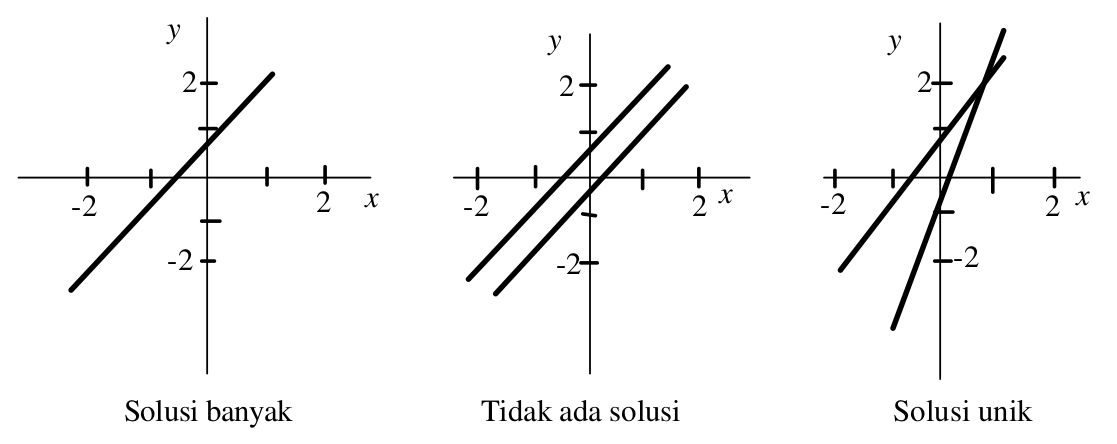
\includegraphics[width=0.9\linewidth]{img/img01}
	\end{center}
\end{frame}

\begin{frame}
	\begin{itemize}
		\item Untuk SPL dengan tiga buah persamaan atau lebih (dengan tiga peubah atau lebih), tidak terdapat tafsiran geometrinya seperti pada SPL dengan dua buah persamaan.
		\item Namun, kita masih dapat memeriksa masing-masing kemungkinan solusi itu berdasarkan pada bentuk matriks akhirnya.
	\end{itemize}
\end{frame}

\begin{frame}
	\frametitle{Solusi unik/tunggal}
	\[
	\left[
		\begin{matrix}
			1 & 1 & 1\\
			2 & 3 & 1\\
			3 & 1 & 2\\
		\end{matrix}
	\right|
	\left.
		\begin{matrix}
			0 \\ 1 \\ 1
		\end{matrix}
	\right]
	\xrightarrow{\text{Eliminasi Gauss}}
	\left[
		\begin{matrix}
			1 & 1 & 1\\
			0 & 1 & -1\\
			0 & 0 & -3\\
		\end{matrix}
	\right|
	\left.
		\begin{matrix}
			0 \\ 1 \\ 3
		\end{matrix}
	\right]
	\]
	Solusi: $ x_1 = 1 $, $ x_2 = 0 $, $ x_3 = -1 $
\end{frame}

\begin{frame}
	\frametitle{Solusi banyak/tidak terhingga}
	\[
	\Scale[0.8]{
	\left[
	\begin{matrix}
	1 & 1 & 2\\
	2 & -1 & 1\\
	1 & 2 & 3\\
	\end{matrix}
	\right|
	\left.
	\begin{matrix}
	4 \\ 2 \\ 6
	\end{matrix}
	\right]
	\xrightarrow{\text{Eliminasi Gauss}}
	\left[
	\begin{matrix}
	1 & 1 & 2\\
	0 & -3 & -3\\
	0 & 0 & 0\\
	\end{matrix}
	\right|
	\left.
	\begin{matrix}
	4 \\ -6 \\ 0
	\end{matrix}
	\right]
	}\]
	\begin{itemize}
		\item Perhatikan hasil eliminasi Gauss pada baris terakhir. Persamaan yang bersesuaian dengan baris terakhir tersebut adalah
		\[ 0x_1 + 0x_2 + 0x_3 = 0 \]
		yang dipenuhi oleh banyak nilai x.
		\item Solusinya diberikan dalam bentuk parameter:
		\item Misalkan $ x_3 = k $ maka $ x_2 = -6 + 3k $ dan $ x_1 = 10-5k $, dengan $ k \in R $
		\item Terdapat tidak berhingga nilai k, berarti solusi SPL banyak sekali.
	\end{itemize}
\end{frame}

\begin{frame}
	\frametitle{Tidak ada solusi}
	\[
	\Scale[0.8]{
		\left[
		\begin{matrix}
		1 & 1 & 2\\
		2 & -1 & 1\\
		1 & 2 & 3\\
		\end{matrix}
		\right|
		\left.
		\begin{matrix}
		4 \\ 2 \\ 7
		\end{matrix}
		\right]
		\xrightarrow{\text{Eliminasi Gauss}}
		\left[
		\begin{matrix}
		1 & 1 & 2\\
		0 & -3 & -3\\
		0 & 0 & 0\\
		\end{matrix}
		\right|
		\left.
		\begin{matrix}
		4 \\ -6 \\ 1
		\end{matrix}
		\right]
	}\]
	\begin{itemize}
		\item Perhatikan hasil eliminasi Gauss pada baris terakhir. Persamaan yang bersesuaian dengan baris terakhir tersebut adalah
		\[ 0x_1 + 0x_2 + 0x_3 = 1 \]
		yang dalam hal ini, tidak nilai $ x_i $ yang memenuhi, $ i = 1, 2, 3 $
	\end{itemize}
\end{frame}

\begin{frame}
	\begin{itemize}
		\item Bentuk akhir matriks setelah eliminasi Gauss untuk ketiga kemungkinan solusi di atas dapat digambarkan sebagai berikut:
	\end{itemize}
	\begin{center}
		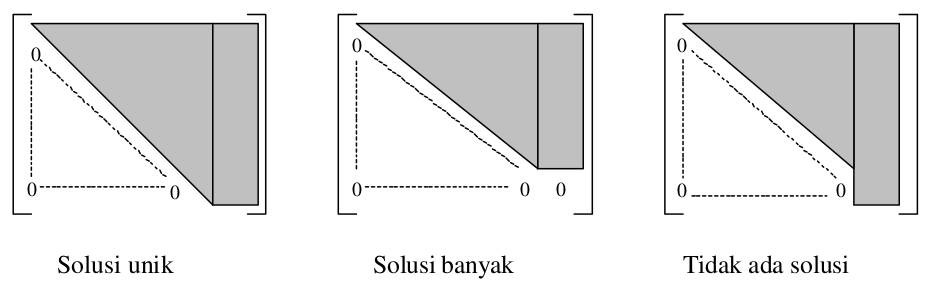
\includegraphics[width=0.9\linewidth]{img/img02}
	\end{center}
\end{frame}

\begin{frame}
	\begin{itemize}
		\item Kita rangkum “pertanda” kemungkinan solusi SPL di bawah ini:
		\begin{enumerate}
			\item Jika pada hasil eliminasi Gauss tidak terdapat baris yang semuanya bernilai 0 (termasuk elemen pada baris yang bersesuaian pada vektor kolom $ b $), maka solusi SPL dipastikan unik.
			\item Jika pada hasil eliminasi Gauss terdapat paling sedikit satu baris yang semuanya bernilai 0 (termasuk elemen pada baris yang bersesuaian pada vektor kolom $ b $), maka SPL mempunyai banyak solusi.
			\item Jika pada hasil eliminasi Gauss terdapat baris yang semuanya bernilai 0 tetapi elemen pada baris yang bersesuaian pada vektor kolom $ b $ tidak 0, maka SPL tidak mempunyai solusi.
		\end{enumerate}
	\end{itemize}
\end{frame}

\section{Metode Eliminasi Gauss-Jordan}

\begin{frame}
	\frametitle{Metode Eliminasi Gauss-Jordan}
	\begin{itemize}
		\item Metode eliminasi Gauss-Jordan merupakan variasi dari metode eliminasi Gauss.
		\item Dalam hal ini, matriks $ A $ dieliminasi menjadi matriks identitas $ I $.
		\[ Ax = b \rightarrow Ix = b' \]
		\item Tidak diperlukan lagi teknik penyulihan mundur untuk memperoleh solusi SPL. Solusinya langsung diperoleh dari vektor kolom $ b $ hasil proses eliminasi.
	\end{itemize}
\end{frame}

\begin{frame}
	\frametitle{Contoh 5}
	\begin{itemize}
		\item \textbf{Persoalan:} Selesaikan sistem persamaan lanjar di bawah ini dengan metode eliminasi Gauss-Jordan.
		\begin{align*}
		3x_1 - 0.1x_2 - 0.2x_3 = 7.85 \\
		0.1x_1 + 7x_2 - 0.3x_3 = -19.3 \\
		0.3x_1 - 0.2x_2 + 10x_3 = 71.4
		\end{align*}
	\end{itemize}
\end{frame}

\begin{frame}
	\begin{itemize}
		\item \textbf{Penyelesaian:}
	\end{itemize}
	\[
	\Scale[0.9]{
	\left[
		\begin{matrix}
			3 & -0.1 & -0.2 \\
			0.1 & 7 & -0.3 \\
			0.3 & -0.2 & 10
		\end{matrix}
	\right|
	\left.
		\begin{matrix}
			7.85 \\ -19.3 \\ 71.4
		\end{matrix}
	\right]
	\begin{matrix}
		R_1 / 3\\
		\\
		\\
	\end{matrix}
	\left[
		\begin{matrix}
			1 & -0.0333333 & -0.0666667 \\
			0.1 & 7 & -0.3 \\
			0.3 & -0.2 & 10
		\end{matrix}
	\right|
	\left.
		\begin{matrix}
			2.61667 \\ -19.3 \\ 71.4
		\end{matrix}
	\right]
	}
	\]
	\[
	\Scale[0.9]{
	\begin{matrix}
		\\
		R_2 - 0.1R_1\\
		R_3 - 0.3R_1
	\end{matrix}
	\left[
		\begin{matrix}
			1 & -0.0333333 & -0.0666667 \\
			0 & 7.00333 & -0.2933333 \\
			0 & -0.190000 & 10.0200
		\end{matrix}
	\right|
	\left.
		\begin{matrix}
			2.61667 \\ -19.5617 \\ 70.6150
		\end{matrix}
	\right]
	}
	\]
	\[
	\Scale[0.9]{
		\begin{matrix}
		\\
		R_2 /7.00333\\
		\\
		\end{matrix}
		\left[
		\begin{matrix}
		1 & -0.0333333 & -0.0666667 \\
		0 & 1 & -0.0418848 \\
		0 & -0.190000 & 10.0200
		\end{matrix}
		\right|
		\left.
		\begin{matrix}
		2.61667 \\ -2.79320 \\ 70.6150
		\end{matrix}
		\right]
	}
	\]
\end{frame}

\begin{frame}
	\[
	\Scale[0.9]{
		\begin{matrix}
		R_1 - (-0.003333)R_2\\
		\\
		R_3 - (-0.190000)R_2
		\end{matrix}
		\left[
		\begin{matrix}
		1 & 0 & -0.0680629 \\
		0 & 1 & -0.0418848 \\
		0 & 0 & 10.01200
		\end{matrix}
		\right|
		\left.
		\begin{matrix}
		2.52356 \\ -2.79320 \\ 70.0843
		\end{matrix}
		\right]
	}
	\]
	\[
	\Scale[0.9]{
		\begin{matrix}
		\\
		\\
		R_3 /10.0200\\
		\end{matrix}
		\left[
		\begin{matrix}
		1 & 0 & -0.0680629 \\
		0 & 1 & -0.0418848 \\
		0 & 0 & 1
		\end{matrix}
		\right|
		\left.
		\begin{matrix}
		2.52356 \\ -2.79320 \\ 7.00003
		\end{matrix}
		\right]
	}
	\]
	\[
	\Scale[0.9]{
		\begin{matrix}
		R_1 - (-0.0680629) R_3\\
		R_2 - (-0.0418848) R_2\\
		\\
		\end{matrix}
		\left[
		\begin{matrix}
		1 & 0 & 0 \\
		0 & 1 & 0 \\
		0 & 0 & 1
		\end{matrix}
		\right|
		\left.
		\begin{matrix}
		3.00000 \\ -2.50001 \\ 7.00003
		\end{matrix}
		\right]
	}
	\]
	\begin{itemize}
		\item Solusi:
		\begin{align*}
			x_1 &= 3.00000 \\
			x_2 &= -2.50001 \\
			x_3 &= 7.00003
		\end{align*}
	\end{itemize}
\end{frame}

\begin{frame}
	\begin{itemize}
		\item Penyelesaian SPL dengan metode eliminasi Gauss-Jordan membutuhkan jumlah komputasi yang lebih banyak daripada metode eliminasi Gauss.
		\item Karena alasan itu, metode eliminasi Gauss sudah cukup memuaskan untuk digunakan dalam penyelesaian SPL.
		\item Namun metode eliminasi Gauss-Jordan merupakan dasar pembentukan matriks balikan (inverse).
	\end{itemize}
\end{frame}

\begin{frame}
	\begin{itemize}
		\item Penyelesaian dengan SPL metode matriks balikan tidak lebih mangkus daripada metode eliminasi Gauss, sebab lebih banyak proses komputasi yang dibutuhkan.
		\item Metode matriks balikan baru mangkus bila digunakan untuk penyelesaian sejumlah SPL dengan matriks A yang sama tetapi dengan vektor kolom b yang berbeda-beda:
		\begin{align*}
			Ax &= b_I \\
			Ax &= b_{II} \\
			Ax &= b_{III} \\
			&\dots \text{dst}
		\end{align*}
		\item Sekali $ A^{-1} $ telah diperoleh, maka ia dapat dipakai untuk
		menyelesaikan sejumlah SPL tersebut.
	\end{itemize}
\end{frame}

\begin{frame}
	\frametitle{Matriks Balikan (inverse matrices)}
	\begin{itemize}
		\item Matriks balikan, $ A^{-1} $ , banyak dipakai dalam pengolahan
		matriks.
		\item Akan ditunjukkan juga bahwa matriks balikan dapat diperoleh dengan metode eliminasi Gauss-Jordan.
		\item Cara analitis untuk menghitung matriks balikan untuk matriks $2 \times 2$:
		\[
		A = 
		\begin{bmatrix}
			a_{11} & a_{12} \\ a_{21} & a_{22}
		\end{bmatrix}
		\rightarrow A^{-1} = \frac{1}{a_{11}a_{22} - a_{12}a_{21}}
		\begin{bmatrix}
			a_{22} & -a_{12} \\ -a_{21} & a_{11}
		\end{bmatrix}
		\]
	\end{itemize}
\end{frame}

\begin{frame}
	\begin{itemize}
		\item Nilai $ a_{11} a_{22} - a_{21}a_{12} $ ini disebut \textbf{determinan}.
		\item Determinan dilambangkan dengan dua buah garis tegak $ (| |) $.
		\item Bila determinan $ A = 0 $, matriks A tidak mempunya balikan, sehingga dinamakan \textit{matriks singular}.
		\item Sistem persamaan lanjar yang mempunyai matriks A singular (sistem singular) tidak mempunyai solusi yang unik, yaitu solusinya banyak atau solusinya tidak ada.
	\end{itemize}
\end{frame}

\begin{frame}
	\begin{itemize}
		\item Untuk matriks $ n \times n $, matriks balikannya dapat diperoleh dengan metode eliminasi Gauss-Jordan, yaitu:
	\end{itemize}
	\[
		\begin{matrix}
			\left[ A \right|
			\left. I \right]
		\end{matrix}
		\rightarrow
		\begin{matrix}
			\left[ I \right|
			\left. A^{-1} \right]
		\end{matrix}
	\]
	\begin{itemize}
		\item[] maka
	\end{itemize}
	\[\Scale[0.9]{
		\left[
			\begin{matrix}
				a_{11} & a_{12} & \dots & a_{1n} \\
				a_{21} & a_{22} & \dots & a_{2n} \\
				\vdots &  &  & \vdots \\
				a_{n1} & a_{n2} & \dots & a_{nn}
			\end{matrix}
		\right|
		\left.
			\begin{matrix}
			1 & 0 & \dots & 0 \\
			0 & 1 & \dots & 0 \\
			\vdots &  &  & \vdots \\
			0 & 0 & \dots & 1
			\end{matrix}
		\right]
		\rightarrow
		\left[
		\begin{matrix}
			1 & 0 & \dots & 0 \\
			0 & 1 & \dots & 0 \\
			\vdots &  &  & \vdots \\
			0 & 0 & \dots & 1
		\end{matrix}
		\right|
		\left.
		\begin{matrix}
			p_{11} & p_{12} & \dots & p_{1n} \\
			p_{21} & p_{22} & \dots & p_{2n} \\
			\vdots &  &  & \vdots \\
			p_{n1} & p_{n2} & \dots & p_{nn}
		\end{matrix}
		\right]
	}\]
\end{frame}

\begin{frame}
	\frametitle{Contoh 6}
	\begin{itemize}
		\item \textbf{Persoalan:} Tentukan matriks balikan dari matriks $ A $ berikut
		\[ A = \begin{bmatrix}
			1 & -1 & 2 \\
			3 & 0 & 1 \\
			1 & 0 & 2
		\end{bmatrix} \]
	\end{itemize}
\end{frame}

\begin{frame}
	\begin{itemize}
		\item \textbf{Penyelesaian:}
	\end{itemize}
	\[
	\left[
		\begin{matrix}
			1 & -1 & 2 \\
			3 & 0 & 1 \\
			1 & 0 & 2
		\end{matrix}
	\right|
	\left.
		\begin{matrix}
			1 & 0 & 0 \\
			0 & 1 & 0 \\
			0 & 0 & 1
		\end{matrix}
	\right]
	\begin{matrix}
		\\
		R_2 - 3R_1 \\
		R_3 - R_1
	\end{matrix}
	\left[
		\begin{matrix}
			1 & -1 & 2 \\
			0 & 3 & -5 \\
			0 & 1 & 0
		\end{matrix}
	\right|
	\left.
		\begin{matrix}
			1 & 0 & 0 \\
			3 & 1 & 0 \\
			1 & 0 & 1
		\end{matrix}
	\right]
	\]
	\[
	\cdots
	\left[
		\begin{matrix}
		1 & 0 & 0 \\
		0 & 1 & 0 \\
		0 & 0 & 1
		\end{matrix}
	\right|
	\left.
		\begin{matrix}
		0 & 0.4 & -0.2 \\
		-1 & 0 & 1 \\
		0 & -0.5 & 0.6
		\end{matrix}
	\right]
	\]
	\begin{itemize}
		\item[] Jadi, matriks balikan dari $ A $ adalah
	\end{itemize}
	\[
	A^{-1} = 
	\begin{bmatrix}
		0 & 0.4 & -0.2 \\
		-1 & 0 & 1 \\
		0 & -0.5 & 0.6
	\end{bmatrix}
	\]
\end{frame}

\section{Metode Matriks Balikan}

\begin{frame}
	\frametitle{Metode Matriks Balikan}
	\begin{itemize}
		\item Misalkan $ A^{-1} $ adalah matriks balikan dari A. Sistem persamaan lanjar $ Ax = b $ dapat diselesaikan sebagai berikut:
		\begin{align*}
			Ax &= b \\
			A^{-1}Ax &= A^{-1}b \\
			Ix &= A^{-1}b \qquad (A^{-1}A = I)\\
			x &= A^{-1}b
		\end{align*}
		\item Cara penyelesaian dengan mengalikan matriks $ A^{-1} $ dengan $ b $ itu dinamakan \textbf{metode matriks balikan}.
	\end{itemize}
\end{frame}

\begin{frame}
	\frametitle{Contoh 7}
	\begin{itemize}
		\item \textbf{Persoalan:} Selesaikan sistem persamaan lanjar
		\begin{align*}
			x_1 - x_2 + 2x_3 &= 5 \\
			3x_1 + x_3 &= 10 \\
			x_1 + 2x_3 &= 5
		\end{align*}
		dengan metode matriks balikan.
	\end{itemize}
\end{frame}

\begin{frame}
	\begin{itemize}
		\item \textbf{Penyelesain:}
		\[
			\left[
				\begin{matrix}
					1 & -1 & 2 \\
					3 & 0 & 1 \\
					1 & 0 & 2 \\
				\end{matrix}
			\right|
			\left.
				\begin{matrix}
					1 & 0 & 0 \\
					0 & 1 & 0 \\
					0 & 0 & 1 \\
				\end{matrix}
			\right]
			\begin{matrix}
				\\
				R_2 - 3R_1 \\
				R_3 - R_1\\
			\end{matrix}
			\left[
				\begin{matrix}
					1 & -1 & 2 \\
					0 & 3 & -5 \\
					0 & 1 & 0 \\
				\end{matrix}
			\right|
			\left.
				\begin{matrix}
					1 & 0 & 0 \\
					-3 & 1 & 0 \\
					-1 & 0 & 1 \\
				\end{matrix}
			\right]
		\]
		\[
		\dots
		\left[
			\begin{matrix}
				1 & 0 & 0 \\
				0 & 1 & 0 \\
				0 & 0 & 1 \\
			\end{matrix}
		\right|
		\left.
			\begin{matrix}
				0 & 0.4 & -0.2 \\
				-1 & 0 & 1 \\
				0 & -0.2 & 0.6 \\
			\end{matrix}
		\right]
		\]
	\end{itemize}
\end{frame}

\begin{frame}
	\begin{itemize}
		\item Solusinya adalah $ x = A^{-1}b $
	\end{itemize}
	\[
		\begin{bmatrix}
		x_1\\ x_2 \\ x_3
		\end{bmatrix}
		=
		\begin{bmatrix}
			0 & 0.4 & -0.2 \\
			-1 & 0 & 1 \\
			0 & -0.2 & 0.6 \\
		\end{bmatrix}
		\begin{bmatrix}
		5 \\ 10 \\ 5
		\end{bmatrix}
		=
		\begin{bmatrix}
		0 + 4 -1 \\
		-5 + 0 + 5 \\
		0 - 2 + 3 \\
		\end{bmatrix}
		=
		\begin{bmatrix}
		3 \\ 0 \\ 1
		\end{bmatrix}
	\]
\end{frame}

\section{Metode Dekomposisi LU}

\begin{frame}
	\frametitle{Metode Dekomposisi LU}
	\begin{itemize}
		\item Jika matriks $ A $ \textit{non-singular} maka ia dapat difaktorkan (diuraikan atau di-dekomposisi) menjadi matriks segitiga bawah L (\textit{lower}) dan matriks segitiga atas U (\textit{upper}):
	\end{itemize}
	\[ A = LU \]
	\[\Scale[0.8]{
	\begin{bmatrix}
		a_{11} & a_{12} & a_{13} & \dots & a_{1n} \\
		a_{21} & a_{22} & a_{23} & \dots & a_{2n} \\
		a_{31} & a_{32} & a_{33} & \dots & a_{3n} \\
		\vdots \\
		a_{n1} & a_{n2} & a_{n3} & \dots & a_{nn} \\
	\end{bmatrix}
	=
	\begin{bmatrix}
		1 & 0 & 0 & \dots & 0 \\
		l_{21} & 1 & 0 & \dots & 0 \\
		l_{31} & l_{32} & 1 & \dots & 0 \\
		\vdots \\
		l_{n1} & l_{n2} & l_{n3} & \dots & 1 \\
	\end{bmatrix}
	\begin{bmatrix}
		u_{11} & u_{12} & u_{13} & \dots & u_{1n} \\
		0 & u_{22} & u_{23} & \dots & u_{2n} \\
		0 & 0 & u_{33} & \dots & u_{3n} \\
		\vdots \\
		0 & 0 & 0 & \dots & u_{nn} \\
	\end{bmatrix}
	}\]
\end{frame}

\begin{frame}
	\begin{itemize}
		\item Sebagai contoh, matriks $3 \times 3$ di bawah ini difaktorkan menjadi:
		\[
		\begin{bmatrix}
			2 & -1 & -1 \\
			0 & -4 & 2 \\
			6 & -3 & 1 \\
		\end{bmatrix}
		=
		\begin{bmatrix}
			1 & 0 & 0 \\
			0 & 1 & 0 \\
			3 & 0 & 1 \\
		\end{bmatrix}
		\begin{bmatrix}
			2 & -1 & -1 \\
			0 & -4 & 2 \\
			0 & 0 & 4 \\
		\end{bmatrix}
		\]
		\item Sekali $ A $ difaktorkan menjadi $ L $ dan $ U $, kedua matriks tersebut dapat digunakan untuk menyelesaikan $ Ax = b $.
		\item Metode penyelesaian SPL dengan cara ini dikenal dengan nama \textbf{metode dekomposisi LU}.
		\item Metode ini dinamakan juga \textbf{metode pemfaktoran segitiga} (\textit{triangular factorization}).
	\end{itemize}
\end{frame}

\begin{frame}
	\begin{itemize}
		\item Tinjau sistem persamaan lanjar \[Ax = b\]
		\item Faktorkan $ A $ menjadi $ L $ dan $ U $ sedemikian sehingga \[ A - LU \]
		\item Jadi, \[Ax = b \rightarrow LUx = b\]
		\item Misalkan \[ Ux = y \]
		maka \[ Ly = b \]
	\end{itemize}
\end{frame}

\begin{frame}
	\begin{itemize}
		\item Untuk memperoleh $ y_1 $, $ y_2 $, $\dots$, $ y_n $, kita menggunakan teknik penyulihan maju (\textit{forward substitution}):
		\[
		\Scale[0.8]{
			Ly = b \rightarrow \begin{bmatrix}
			1 & 0 & 0 & \dots & 0\\
			l_{21} & 1 & 0 & \dots & 0\\
			\vdots & \vdots & \vdots & \vdots & \vdots\\
			l_{n1} & l_{n2} & l_{n3} & \dots & 0\\
			\end{bmatrix}
			\begin{bmatrix}
			y_1 \\ y_2 \\ \vdots \\ y_n
			\end{bmatrix}
			=
			\begin{bmatrix}
			b_1 \\ b_2 \\ \vdots \\ b_n
			\end{bmatrix}
			\rightarrow 
			\begin{matrix}
			\text{diperoleh}& \\
			y_1 , y_2 ,\dots, y_n&\\
			\text{dengan teknik}&\\
			\text{penyulihan maju}&
			\end{matrix}
		}\]
		\item Dan untuk memperoleh solusi SPL, $ x_1 $, $ x_2 $, $ \dots $, $ x_n $, kita menggunakan teknik penyulihan mundur (\textit{backward substitution}):
		\[
		\Scale[0.8]{
			Ux = y \rightarrow \begin{bmatrix}
			u_{11} & u_{12} & u_{13} & \dots & u_{1n}\\
			0 & u_{22} & u_{23} & \dots & u_{2n}\\
			\vdots & \vdots & \vdots & \vdots & \vdots\\
			0 & 0 & 0 & \dots & u_{nm}\\
			\end{bmatrix}
			\begin{bmatrix}
			x1 \\ x_2 \\ \vdots \\ x_n
			\end{bmatrix}
			=
			\begin{bmatrix}
			y_1 \\ y_2 \\ \vdots \\ y_n
			\end{bmatrix}
			\rightarrow 
			\begin{matrix}
			\text{diperoleh}& \\
			x_1 , x_2 ,\dots, x_n&\\
			\text{dengan teknik}&\\
			\text{penyulihan mundur}&
			\end{matrix}
		}\]
	\end{itemize}
\end{frame}

\begin{frame}
	\begin{itemize}
		\item Jadi, langkah-langkah menghitung solusi SPL dengan metode dekomposi LU dapat diringkas sebagai berikut:
		\begin{enumerate}
			\item Bentuklah matriks $ L $ dan $ U $ dari $ A $
			\item Pecahkan $ Ly = b $, lalu hitung $ y $ dengan teknik penyulihan maju
			\item Pecahkan $ Ux = y $, lalu hitung $ x $ dengan teknik penyulihan mundur
		\end{enumerate}
		\item Terdapat dua metode untuk memfaktorkan A atas L dan U:
		\begin{enumerate}
			\item Metode LU Gauss.
			\item Metode reduksi Crout.
		\end{enumerate}
	\end{itemize}
\end{frame}

\subsection{Pemfaktoran dengan Metode LU Gauss}

\begin{frame}
	\frametitle{Pemfaktoran dengan Metode\\LU Gauss}
	\begin{itemize}
		\item Misalkan matriks $ A $ berukuran $ 4 \times 4 $ difaktorkan atas $ L $ dan $ U $,
		\[A = LU\]
		\[\Scale[0.8]{
			\begin{bmatrix}
				a_{11} & a_{12} & a_{13} & a_{14} \\
				a_{21} & a_{22} & a_{23} & a_{24} \\
				a_{31} & a_{32} & a_{33} & a_{34} \\
				a_{41} & a_{42} & a_{43} & a_{44} \\
			\end{bmatrix}
			=
			\begin{bmatrix}
			1 & 0 & 0 & 0 \\
			m_{21} & 1 & 0 & 0 \\
			m_{31} & m_{32} & 1 & 0 \\
			m_{41} & m_{42} & m_{43} & 1 \\
			\end{bmatrix}
			\begin{bmatrix}
			u_{11} & u_{12} & u_{13} & u_{14} \\
			0 & u_{22} & u_{23} & u_{24} \\
			0 & 0 & u_{33} & u_{34} \\
			0 & 0 & 0 & u_{44} \\
			\end{bmatrix}
		}\]
		\item Di sini kita menggunakan simbol $ m_{ij} $ ketimbang $ l_{ij} $ , karena nilai $ l_{ij} $ berasal dari faktor pengali ($ l_{ij} $) pada proses eliminasi Gauss.
		\item Langkah-langkah pembentukan $ L $ dan $ U $ dari matriks $ A $ adalah sebagai berikut:
	\end{itemize}
\end{frame}

\begin{frame}
	\begin{enumerate}
		\item Nyatakan $ A $ sebagai $ A = IA $
		\[\Scale[0.8]{
		\begin{bmatrix}
			a_{11} & a_{12} & a_{13} & \dots & a_{1n}\\
			a_{21} & a_{22} & a_{23} & \dots & a_{2n}\\
			a_{31} & a_{32} & a_{33} & \dots & a_{3n}\\
			\vdots & \vdots & \vdots & \dots & \vdots\\
			a_{n1} & a_{n2} & a_{n3} & \dots & a_{nn}
		\end{bmatrix}
		=
		\begin{bmatrix}
			1 & 0 & 0 & \dots & 0\\
			0 & 1 & 0 & \dots & 0\\
			0 & 0 & 1 & \dots & 0\\
			\vdots & \vdots & \vdots & \dots & \vdots\\
			0 & 0 & 0 & \dots & 1
		\end{bmatrix}
		\begin{bmatrix}
			a_{11} & a_{12} & a_{13} & \dots & a_{1n}\\
			a_{21} & a_{22} & a_{23} & \dots & a_{2n}\\
			a_{31} & a_{32} & a_{33} & \dots & a_{3n}\\
			\vdots & \vdots & \vdots & \dots & \vdots\\
			a_{n1} & a_{n2} & a_{n3} & \dots & a_{nn}
		\end{bmatrix}
		}\]
		\item Eliminasikan matriks $ A $ di ruas kanan menjadi matriks segitiga atas $ U $.
		Tempatkan faktor pengali $ m_{ij} $ pada posisi $ l_{ij} $ di matriks $ I $.
		\item Setelah seluruh proses eliminasi Gauss selesai, matriks $ I $ menjadi matriks $ L $, dan matriks $ A $ di ruas kanan menjadi matriks $ U $.
	\end{enumerate}
\end{frame}

\begin{frame}
	\frametitle{Contoh 8}
	\begin{itemize}
		\item \textbf{Persoalan LU Gauss naif:} Faktorkan matriks $ A $ berikut dengan metode LU Gauss.
		\[ A = 
		\begin{bmatrix}
			4 & 3 & -1\\
			-2 & -4 & 5\\
			1 & 2 & 6\\
		\end{bmatrix}
		\]
	\end{itemize}
\end{frame}

\begin{frame}
	\begin{itemize}
		\item \textbf{Penyelesaian:}
		\[\Scale[0.7]{ A = 
		\begin{bmatrix}
			4 & 3 & -1\\
			-2 & -4 & 5\\
			1 & 2 & 6\\
		\end{bmatrix}
		=
		\begin{bmatrix}
			1 & 0 & 0\\
			0 & 1 & 0\\
			0 & 0 & 1\\
		\end{bmatrix}
		\begin{bmatrix}
			4 & 3 & -1\\
			-2 & -4 & 5\\
			1 & 2 & 6\\
		\end{bmatrix}
		}\]
		\item Eliminasikan matriks $ A $ di ruas kanan menjadi matriks segitiga atas $ U $, dan tempatkan faktor pengali $ m_{ij} $ pada posisi $ l_{ij} $ di matriks $ I $.
		\[\Scale[0.7]{
		\begin{bmatrix}
			4 & 3 & -1\\
			-2 & -4 & 5\\
			1 & 2 & 6\\
		\end{bmatrix}
		\begin{matrix}
			\\
			R_2 - (-2/4)R_1\\
			R_3 - (1/4)R_1
		\end{matrix}
		\begin{bmatrix}
			4 & 3 & -1\\
			0 & -2.5 & 4.5\\
			0 & 1.25 & 6.25\\
		\end{bmatrix}
		}\]
		\item Tempatkan $ m_{21} = -2/4 = -0.5 $ dan $ m_{31} = 1/4 = 0.25 $ ke dalam matriks $ L $:
		\[\Scale[0.7]{ L = 
		\begin{bmatrix}
			1 & 0 & 0\\
			-0.5 & 1 & 0\\
			0.25 & m_{32} & 1\\
		\end{bmatrix}
		}\]
	\end{itemize}
\end{frame}

\begin{frame}
	\begin{itemize}
		\item Teruskan proses eliminasi Gauss pada matriks $ A $,
		\[\Scale[0.7]{
		\begin{bmatrix}
			4 & 3 & -1 \\
			0 & -2.5 & 4.5 \\
			0 & 1.25 & 6.25 \\
		\end{bmatrix}
		\begin{matrix}
			\\\\R_3 - (1.25/-2.5)R_2
		\end{matrix}
		\begin{bmatrix}
			4 & 3 & -1 \\
			0 & -2.5 & 4.5 \\
			0 & 0 & 8.5 \\
		\end{bmatrix}
		=U
		}\]
		\item Tempatkan $ m_{32} = 1.25/-2.5 = -0.5 $ ke dalam matriks $ L $:
		\[\Scale[0.7]{ L = 
		\begin{bmatrix}
			1 & 0 & 0 \\
			-0.5 & 1 & 0 \\
			0.25 & -0.5 & 1 \\
		\end{bmatrix}
		}\]
		\item Jadi,
		\[\Scale[0.7]{ A = 
		\begin{bmatrix}
			4 & 3 & -1\\
			-2 & -4 & 5\\
			1 & 2 & 6\\
		\end{bmatrix} = 
		\begin{bmatrix}
			1 & 0 & 0 \\
			-0.5 & 1 & 0 \\
			0.25 & -0.5 & 1 \\
		\end{bmatrix}
		\begin{bmatrix}
		4 & 3 & -1 \\
		0 & -2.5 & 4.5 \\
		0 & 0 & 8.5 \\
		\end{bmatrix}
		}\]
	\end{itemize}
\end{frame}

\begin{frame}
	\frametitle{Contoh 9}
	\begin{itemize}
		\item \textbf{Persoalan LU Gauss tata-ancang pivoting:} Faktorkan matriks A berikut
		\[ A = \begin{bmatrix}
		1 & 1 & -1 \\
		2 & 2 & -1 \\
		-1& 1 & 1 \\
		\end{bmatrix}
		\qquad
		b = \begin{bmatrix}
		1 \\ 5 \\ 1
		\end{bmatrix}
		\]
		lalu pecahkan sistem $ Ax = b $.
	\end{itemize}
\end{frame}

\begin{frame}
	\begin{itemize}
		\item \textbf{Penyelesaian:} Eliminasikan matriks $ A $ di ruas kanan menjadi matriks segitiga atas $ U $, dan tempatkan faktor pengali $ m_{ij} $ pada posisi $ l_{ij} $ di matriks $ I $
		\[ \begin{bmatrix}
			\textbf{1} & 1 & -1 \\
			2 & 2 & 1 \\
			-1 & 1 & 1
		\end{bmatrix}
		\begin{matrix}
		\\ R_2 - 2R_1 \\
		R_3 - (1/1)R_1
		\end{matrix}
		\begin{bmatrix}
		\textbf{1} & 1 & -1 \\
		0 & 0 & 3 \\
		0 & 2 & 0
		\end{bmatrix} \]
		\item Tempatkan $ m_{21} = 2/1 = 2 $ dan $ m_{31} = -1/1 = -1 $ ke dalam matriks $ L $:
		\[ L = \begin{bmatrix}
			1 & 0 & 0 \\
			2 & 1 & 0 \\
			-1 & m_{32} & 1
		\end{bmatrix} \]
	\end{itemize}
\end{frame}

\begin{frame}
	\begin{itemize}
		\item Teruskan proses eliminasi Gauss pada matriks $ A $. Dalam hal ini ada pivoting karena calon pivot bernilai $ 0 $, sehingga baris kedua dipertukarkan dengan baris ketiga:
		\[ \begin{bmatrix}
			1 & 1 & -1 \\
			0 & \textbf{0} & 3 \\
			0 & \textbf{2} & 0
		\end{bmatrix} R_2 \Leftrightarrow R_3
		\begin{bmatrix}
			1 & 1 & -1 \\
			0 & \textbf{2} & 0 \\
			0 & \textbf{0} & 3 \\
		\end{bmatrix}\]
		\item Jangan lupa mempertukarkan juga $ R_2 \Leftrightarrow R_3 $ pada matriks $ L $, kecuali elemen diagonalnya
		\[
		L = \begin{bmatrix}
			1 & 0 & 0 \\
			\textbf{2} & 1 & 0 \\
			\textbf{-1} & m_{32} & 1
		\end{bmatrix}
		R_2 \Leftrightarrow R_3
		\begin{bmatrix}
			1 & 0 & 0 \\
			\textbf{-1} & 1 & 0 \\
			\textbf{2} & m_{32} & 1
		\end{bmatrix}
		\]
	\end{itemize}
\end{frame}

\begin{frame}
	\begin{itemize}
		\item Jangan lupa mempertukarkan juga $ R_2 \Leftrightarrow R_3 $ pada vektor $ b $,
		\[ b = \begin{bmatrix}
		1 \\ \textbf{5} \\ \textbf{1}
		\end{bmatrix} R_2 \Leftrightarrow R_3
		 \begin{bmatrix}
		1 \\ \textbf{1} \\ \textbf{5}
		\end{bmatrix}
		\]
		\item Teruskan proses eliminasi Gauss pada matriks $ A $:
		\[ R_3 - (0/2)R_2 \begin{bmatrix}
			1 & 1 & -1 \\
			0 & \textbf{2} & 0 \\
			0 & 0 & 3
		\end{bmatrix} = U \]
		\item Tempatkan $ m_{32} = 0/2 = 0 $ ke dalam matriks $ L $:
		\[ L = \begin{bmatrix}
			1 & 0 & 0 \\
			-1 & 1 & 0 \\
			2 & 0 & 1
		\end{bmatrix}\]
	\end{itemize}
\end{frame}

\begin{frame}
	\begin{itemize}
		\item Jadi,
		\[\Scale[0.8]{ A = 
		\begin{bmatrix}
			1 & 1 & -1 \\
			-1 & 1 & 1 \\
			2 & 2 & 1
		\end{bmatrix} = 
		\begin{bmatrix}
			1 & 0 & 0 \\
			-1 & 1 & 0 \\
			2 & 0 & 1
		\end{bmatrix}
		\begin{bmatrix}
			1 & 1 & -1\\
			0 & 2 & 0 \\
			0 & 0 & 3
		\end{bmatrix}
		}\]
		\item Berturut-turut dihitung $ y $ dan $ x $ sebagai berikut:
		\[ Ly = b \rightarrow \begin{bmatrix}
		1 & 0 & 0\\
		-1 & 1 & 0\\
		2 & 0 & 1
		\end{bmatrix}
		\begin{bmatrix}
			y_1 \\ y_2 \\ y_3
		\end{bmatrix} = 
		\begin{bmatrix}
			1 & 1 & 5
		\end{bmatrix}\]
		\item $ y_1 $, $ y_2 $, dan $ y_3 $ dihitung dengan teknik penyulihan maju:
		\begin{align*}
			y_1 &= 1\\
			-y_1 + y_2 &= 1 \rightarrow y_2 = 1 + y_1 = 1 + 1 = 2 \\
			2y_1 + 0y_2 + y_3 &= 5 \rightarrow y_3 = 5 - 2y_1 = 3
		\end{align*}
	\end{itemize}
\end{frame}

\begin{frame}
	\[ Ux = y \rightarrow \begin{bmatrix}
	1 & 1 & -1 \\
	0 & 2 & 0 \\
	0 & 0 & 3
	\end{bmatrix}
	\begin{bmatrix}
	x_1 \\ x_2 \\ x_3
	\end{bmatrix} = 
	\begin{bmatrix}
	1 \\ 2 \\ 3
	\end{bmatrix} \]
	
	\begin{itemize}
		\item $ x_1 $, $ x_2 $, dan $ x_3 $ dihitung dengan teknik penyulihan mundur:
		\begin{align*}
			3x_3 &= 3 \leftarrow x_3 = 1 \\
			2x_2 + 0x_3 &= 2 \leftarrow x_2 = 1 \\
			x_1 + x_2 + x_3 &= 1 \leftarrow x_1 = 1
		\end{align*}
		\item Jadi, solusi sistem persamaan lanjar di atas adalah $ x = (1, 1, 1)^T $ .
	\end{itemize}
\end{frame}

\begin{frame}
	\begin{itemize}
		\item Pertukaran baris untuk matriks yang berukuran besar diperlihatkan oleh matriks di bawah ini:
		\[\Scale[0.9]{
		\begin{bmatrix}
			a_1 & a_2 & a_3 & a_4 & a_5 & a_6 \\
			0 & b_2 & b_3 & b_4 & b_5 & b_6 \\
			0 & 0 & c_3 & c_4 & c_5 & c_6 \\
			0 & 0 & 0 & 0 & d_5 & d_6 \\
			0 & 0 & 0 & e_4 & e_5 & e_6 \\
			0 & 0 & 0 & f_4 & f_5 & f_6
		\end{bmatrix}
		R_5 \Leftrightarrow R_4
		\begin{bmatrix}
		a_1 & a_2 & a_3 & a_4 & a_5 & a_6 \\
		0 & b_2 & b_3 & b_4 & b_5 & b_6 \\
		0 & 0 & c_3 & c_4 & c_5 & c_6 \\
		0 & 0 & 0 & e_4 & e_5 & e_6 \\
		0 & 0 & 0 & 0 & d_5 & d_6 \\
		0 & 0 & 0 & f_4 & f_5 & f_6
		\end{bmatrix}
		}\]
	\end{itemize}
\end{frame}

\begin{frame}
	\begin{itemize}
		\item Maka, baris ke-5 dan baris ke-4 pada matriks L juga harus dipertukarkan:
		\[\Scale[0.9]{
		\begin{bmatrix}
			1 & 0 & 0 & 0 & 0 & 0 \\
			m_{21} & 1 & 0 & 0 & 0 & 0 \\
			m_{31} & m_{32} & 1 & 0 & 0 & 0 \\
			m_{41} & m_{42} & m_{43} & 1 & 0 & 0 \\
			m_{51} & m_{52} & m_{53} & x & 1 & 0 \\
			m_{61} & m_{62} & m_{63} & x & x & 1
		\end{bmatrix}
		R_5 \Leftrightarrow R_4
		\begin{bmatrix}
			1 & 0 & 0 & 0 & 0 & 0 \\
			m_{21} & 1 & 0 & 0 & 0 & 0 \\
			m_{31} & m_{32} & 1 & 0 & 0 & 0 \\
			m_{51} & m_{52} & m_{53} & 1 & 0 & 0 \\
			m_{41} & m_{42} & m_{43} & x & 1 & 0 \\
			m_{61} & m_{62} & m_{63} & x & x & 1
		\end{bmatrix}
		}\]
	\end{itemize}
\end{frame}

\subsection{Pemfaktoran dengan Metode Reduksi Crout}

\begin{frame}
	\frametitle{Pemfaktoran dengan Metode Reduksi Crout}
	\begin{itemize}
		\item Meskipun metode $ LU $ Gauss dikenal paling baik untuk melakukan dekomposisi LU, terdapat metode lain yang digunakan secara luas, yaitu \textbf{metode reduksi Crout}
		\item Nama lain: \textbf{metode reduksi Cholesky} atau \textbf{metode Dolittle}
		\item Dalam membahas metode reduksi Crout, tinjau matriks $ 3 \times 3 $ berikut:
		\[\Scale[0.9]{
		A = \begin{bmatrix}
			a_{11} & a_{12} & a_{13} \\
			a_{21} & a_{22} & a_{23} \\
			a_{31} & a_{32} & a_{33} \\
		\end{bmatrix}\quad
		L = \begin{bmatrix}
			1 & 0 & 0 \\
			l_{21} & 1 & 0 \\
			l_{31} & l_{32} & 1 \\
		\end{bmatrix}\quad
		U = \begin{bmatrix}
			u_{11} & u_{12} & u_{13} \\
			0 & u_{22} & u_{23} \\
			0 & 0 & u_{33} \\
		\end{bmatrix}
		}\]
	\end{itemize}
\end{frame}

\begin{frame}
	\begin{itemize}
		\item Karena $ LU = A $, maka hasil perkalian $ L $ dan $ U $ itu dapat ditulis sebagai
	\end{itemize}
	\begin{align*}
		LU &= A \\
		\begin{bmatrix*}[l]
		u_{11} & u_{12} & u_{13} \\
		l_{21}u_{11} & l_{21}u_{12}+u_{22} & l_{21}u_{13}+u_{23} \\
		l_{31}u_{13} & l_{31}u_{12} + l_{32}u_{22}  & l_{31}u_{13} + l_{32}u_{23} + u_{33}\\
		\end{bmatrix*} &= \begin{bmatrix*}[l]
		a_{11} & a_{12} & a_{13} \\
		a_{21} & a_{22} & a_{23} \\
		a_{31} & a_{32} & a_{33} \\
		\end{bmatrix*}
	\end{align*}
\end{frame}

\begin{frame}
	\begin{itemize}
		\item Dari kesamaan dua buah matriks $ LU = A $, diperoleh
		\begin{enumerate}
			\item Baris pertama $ U $ 
			\[ u_{11} = a_{11},~u_{12} = a_{12},~u_{13}=a_{13}\]
			\item Kolom pertama $ L $
			\begin{align*}
				l_{21} u_1 = a_{21} &\rightarrow l_{21} = \frac{a_{21}}{u_{11}} \\
				l_{31} u_{11} = a_{31} &\rightarrow l_{31} = \frac{a_{31}}{u_{11}}
			\end{align*}
			\item Baris kedua $ U $
			\begin{align*}
				l_{21}u_{12} + u_{22} = a_{22} &\rightarrow u_{22} = a_{22} - l_{21}u_{12} \\
				l_{21}u_{13} + u_{23} = a_{23} &\rightarrow u_{23} = a_{23} - l_{21}u_{13}
			\end{align*}
		\end{enumerate}
	\end{itemize}
\end{frame}

\begin{frame}
	\begin{itemize}
		\item Dari kesamaan dua buah matriks $ LU = A $, diperoleh
		\begin{enumerate}
			\setcounter{enumi}{3}
			\item Kolom kedua $ L $
			\[ l_{31}u_{12} + l_{32}u_{22} = a_{32} \rightarrow l_{32} = \frac{a_{32}-l_{31}u_{12}}{u_{22}} \]
			\item Baris ketiga $ U $
			\[ l_{31}u_{13} + l_{32}u_{23} + u_{33} = a_{33} \rightarrow u_{33} = a_{33} - (l_{31}u_{13} - l_{32}u_{23}) \]
		\end{enumerate}
	\end{itemize}
\end{frame}

\begin{frame}
	\begin{itemize}
		\item Kita perhatikan ada urutan pola teratur dalam menemukan
		elemen-elemen $ L $ dan $ U $, yaitu:
		\begin{enumerate}
			\item elemen-elemen baris pertama dari $ U $
			\item elemen-elemen baris pertama dari $ L $
			\item elemen-elemen baris kedua dari $ U $
			\item elemen-elemen baris kedua $ L $
			\item[] $ \vdots $
			\item elemen-elemen baris ke-$ k $ dari $ U $
			\item elemen-elemen baris ke-$ k $ dari $ L $
		\end{enumerate}
	\end{itemize}
\end{frame}

\begin{frame}
	\begin{itemize}
		\item Rumus umum menghitung $ u $ dan $ l $ untuk sistem dengan matriks $ A $ yang berukuran $ 3 \times 3 $ dapat ditulis sebagai berikut:
		\[ u_{pj} = a_{pj} - \sum_{k=1}^{p-1}l_{pk}u_{kj},\qquad
		\begin{matrix}
			p &= 1,2,3,\dots,n \\
			j &= p,p+1,\dots,n \\
		\end{matrix} \]
		dan
		\[ l_{iq} = \frac{a_{iq} - \sum_{k=1}^{q-1}l_{ik}u_{kq}}{u_{qq}},\qquad
		\begin{matrix}
		q &= 1,2,3,\dots,n-1 \\
		i &= q+1,q+2,\dots,n \\
		&\text{ dengan syarat } u_{qq} \neq 0
		\end{matrix} \]
	\end{itemize}
\end{frame}

\begin{frame}
	\frametitle{Contoh 10}
	\begin{itemize}
		\item \textbf{Persoalan:} Selesaikan
		\begin{align*}
			x_1 + x_2 - x_3 &= 1 \\
			2x_1 + 2x_2 + x_3 &= 5 \\
			-x_1 + x_2 + 2x_3 &= 5
		\end{align*}
		dengan metode dekomposisi $ LU $, yang dalam hal ini $ L $ dan $ U $ dihitung dengan metode reduksi Crout.
	\end{itemize}
\end{frame}

\begin{frame}
	\begin{itemize}
		\item \textbf{Penyelesaian:}
		\[ A = \begin{bmatrix}
		1 & 1 & -1 \\ 2 & 2 & 1 \\ -1 & 1 & 1
		\end{bmatrix}\qquad b = \begin{bmatrix}
		1 \\ 5 \\ 1
		\end{bmatrix} \]
		\item[] diperoleh
		\begin{align*}
			u_{11} &= a_{11} = 1 \\
			u_{12} &= a_{12} = 1 \\
			u_{13} &= a_{13} = -1 \\
			\\
			l_{21} &= a_{21}/u_{11} = 2/1 = 2 \\
			l_{31} &= a_{31}/u_{11} = -1/1 = -1 \\
		\end{align*}
	\end{itemize}
\end{frame}

\begin{frame}
	\begin{itemize}
		\item[]
		\begin{align*}
			u_{22} &= a_{22} - l_{21}u_{12} = 2 - 2(1) = 0 \\
		\end{align*}
		\item Karena $ u_{qq} $ tidak boleh nol, lakukan pertukaran baris, baik untuk matriks $ A $ maupun untuk vektor $ b $:
		\[
		A = R_2 \Leftrightarrow R_3 \begin{bmatrix}
		1 & 1 & -1\\ -1 & 1 & 1 \\ 2 & 2 & 1 
		\end{bmatrix} \qquad R_2 \Leftrightarrow b = R_3\begin{bmatrix}
		1 \\ 1 \\ 5 
		\end{bmatrix}
		\]
		\item Hitung kembali nilai $ l_{21} $ , $ l_{31} $ , dan $ u_{22} $ (Perhatikan bahwa nilai $ u_{11} $ , $ u_{12} $ , $ u_{13} $ tidak berubah)
	\end{itemize}
\end{frame}

\begin{frame}
	\begin{itemize}
		\item[]
		\begin{align*}
		l_{21} &= a_{21}/u_{11} = -1/1 = -1 \\
		l_{31} &= a_{31}/u_{11} = 2/1 = 2 \\
		\\
		u_{22} &= a_{22} - l_{21}u_{12} = 1-(-1)(1) = 2 \\
		u_{23} &= a_{23} - l_{21}u_{13} = 1-(-1)(-1) = 0 \\
		\\
		l_{32} &= \frac{a_{32}-l_{31}u_{12}}{u_{22}} = \frac{2-2(1)}{2} = 0
		\\
		u_{33} &= a_{33} - (l_{31}u_{13}+l_{32}u_{23}) = 1 - [2\cdot(-1) + 0\cdot0] = 3
		\end{align*}
	\end{itemize}
\end{frame}

\begin{frame}
	\begin{itemize}
		\item Diperoleh $ L $ dan $ U $ sebagai berikut,
		\[U = \begin{bmatrix}
		1 & 1 & -1 \\ 0 & 2 & 0 \\ 0 & 0 & 3
		\end{bmatrix}\quad L = \begin{bmatrix}
		1 & 0 & 0 \\ -1 & 1 & 0 \\ 2 & 0 & 1
		\end{bmatrix} \text{ dan } b = \begin{bmatrix}
		1 \\ 1 \\ 5
		\end{bmatrix}\]
		\item Berturut-turut dihitung $ y $ dan $ x $ sebagai berikut:
		\[ Ly = b \rightarrow \begin{bmatrix}
		1 & 0 & 0 \\ -1 & 1 & 0 \\ 2 & 0 & 1
		\end{bmatrix} \begin{bmatrix}
		y_1 \\ y_2 \\ y_3
		\end{bmatrix} = \begin{bmatrix}
		1 \\ 1 \\ 5
		\end{bmatrix}\]
	\end{itemize}
\end{frame}

\begin{frame}
	\begin{itemize}
		\item $ y_1 $, $ y_2 $, dan $ y_3 $ dihitung dengan teknik penyulihan maju:
		\begin{align*}
			y_1 &= 1 \\
			-y_1 + y_2 &= 1 \rightarrow y_2 = 1 + y_1 = 1 + 1 = 2 \\
			2y_1 + 0y_2 + y_3 &= 5 \rightarrow y_3 = 5 - 2y_1 = 3
		\end{align*}
	\end{itemize}
\end{frame}

\begin{frame}
	\begin{itemize}
		\item[] 
		\[ Ux = y \rightarrow \begin{bmatrix}
		1 & 1 & -1 \\ 0 & 2 & 0 \\ 0 & 0 & 3
		\end{bmatrix} \begin{bmatrix}
		x_1 \\ x_2 \\ x_3
		\end{bmatrix} = \begin{bmatrix}
		1 \\ 2 \\ 3
		\end{bmatrix}\]
		\item $ x_1 $, $ x_2 $, dan $ x_3 $ dihitung dengan teknik penyulihan mundur:
		\begin{align*}
		3x_3 &= 3 \rightarrow x_3 = 1 \\
		2x_2 + 0x_3 &= 2 \rightarrow x_2 = 1 \\
		x_1 + x_2 - x_3 &= 1 \rightarrow x_1 = 1
		\end{align*}
		\item Jadi, solusi sistem persamaan lanjar di atas adalah $ x = (1, 1, 1)^T $.
	\end{itemize}
\end{frame}

\begin{frame}
	\begin{itemize}
		\item Jika diamati elemen segitiga bawah pada matriks $ U $ semuanya bernilai nol, sehingga ruang yang tidak terpakai itu dapat dipakai untuk menyimpan elemen matriks $ L $.
		\item Elemen diagonal matriks $ L $ seluruhnya 1, jadi tidak perlu disimpan (\textit{default}). Dengan demikian, penyimpanan elemen $ L $ dan $ U $ pada satu matriks dapat menghemat penggunaan memori.
		\item Selain itu, matriks $ A $ hanya dipakai sekali untuk
		memperoleh $ L $ dan $ U $, sesudah itu tidak dipakai lagi.
		\item Dengan demikian, setelah $ L $ dan $ U $ diperoleh, elemennya dapat dipindahkan ke dalam $ A $.
		\item Karena alasan ini, maka metode dekomposisi $ LU $ dinamakan juga metode kompaksi memori.
	\end{itemize}
\end{frame}

\section{Determinan}

\begin{frame}
	\frametitle{Determinan}
	\begin{itemize}
		\item Metode eliminasi Gauss dapat diterapkan untuk menghitung
		determinan matriks $ n \times n $.
		\item Determinannya dapat dihitung setelah ia ditransformasi menjadi matriks segitiga atas $ U $.
		\item Dua hukum penting determinan:
		\begin{itemize}
			\item $ det(BC) = det(B) \times det(C) $
			\item $ det(M) = $ hasil kali semua elemen diagonal $ M $ jika $ M $ adalah matriks segitiga atas atau matriks segitiga
			bawah.
		\end{itemize}
	\end{itemize}
\end{frame}

\begin{frame}
	\frametitle{Kasus 1: Bila eliminasi Gauss tidak menerapkan tata-ancang pivoting.}
	\begin{itemize}
		\item Jika pivoting tidak diterapkan, determinan matriks $ A $
		adalah:
		\begin{align*}
			det(A) &= det(LU) \\
			&= det(L) \times det(U) \\
			&= det(U) \\
			&= u_{11}u_{22}u_{33} \dots u_{nn}
		\end{align*}
		\item yang dalam hal ini $ det(L) = 1 $ sebab semua elemen diagonal $ L $ adalah satu.
	\end{itemize}
\end{frame}

\begin{frame}
	\frametitle{Kasus 1: Bila eliminasi Gauss menerapkan tata-ancang pivoting.}
	\begin{itemize}
		\item Tatancang pivoting mengakibatkan pertukaran baris.
		\item Dekomposisi LU dengan pivoting setara dengan mengerjakan dua proses terpisah berikut:
		\begin{enumerate}
			\item Transformasikan matriks $ A $ menjadi matriks $ A' $ dengan cara permutasi baris-baris matriks (sama dengan mengalikan $ A $ dengan matriks permutasi $ P $),
			\[ A' = PA \] atau setara dengan \[ A = P^{-1}A' \]
			\item Dekomposisi $ A' $ menjadi $ LU $ tanpa pivoting
			\[A' = LU\]
		\end{enumerate}
	\end{itemize}
\end{frame}

\begin{frame}
	\begin{itemize}
		\item Dari (1) dan (2), $ L $ dan $ U $ dihubungkan dengan $ A $ oleh
		\[ A = P -1 A' = P -1 LU \]
		\item Determinan $ A $ dapat ditulis sebagai
		\begin{align*}
			det(A) &= det(P^{-1}) \times det(L) \times det(U) \\
			&= det(P^{-1}) \times 1 \times det(U) \\
			&= det(P^{-1}) \times det(U) \\
			&= \alpha det(U)
		\end{align*}
		\item yang dalam hal ini $ \alpha = det(P^{-1}) = -1 $ atau $ 1 $ bergantung pada apakah pivoting sejumlah bilangan ganjil atau genap.
	\end{itemize}
\end{frame}

\begin{frame}
	\begin{itemize}
		\item Jika pivoting dilakukan sejumlah $ p $ kali, maka $\alpha$ dapat ditulis sebagai:
		$ \alpha = (-1)^p $
		\item $\alpha$ bernilai 1 untuk $ p $ genap dan -1 untuk$  p $ ganjil. Karena itu,
		\[ det(A) = (-1)^pdet(U) = (-1)^p u_{11} u_{22} u_{33} \dots u_{nn} \]
	\end{itemize}
\end{frame}

\begin{frame}
	\frametitle{Contoh 11}
	\begin{itemize}
		\item \textbf{Persoalan:} Hitung determinan matriks $ A $ berikut:
		\[ A = \begin{bmatrix}
		2 & 3 & -1 \\ 4 & 4 & -3 \\ -2 & 3 & -1
		\end{bmatrix} \]
	\end{itemize}
\end{frame}

\begin{frame}
	\frametitle{Contoh 11}
	\begin{itemize}
		\item \textbf{Penyelesaian:}
		\[ \begin{bmatrix}
		2 & 3 & -1 \\ 4 & 4 & -3 \\ -2 & 3 & -1
		\end{bmatrix}
		\begin{matrix}
		R_2 - \frac{4}{2}R_1 \\
		R_3 - \frac{-2}{2}R_1 \\
		\end{matrix}
		\begin{bmatrix}
		2 & 3 & -1 \\ 0 & -2 & -1 \\ 1 & 0 & -2
		\end{bmatrix}
		\begin{matrix}
		R_3 - \frac{6}{-2}R_2
		\end{matrix}
		\begin{bmatrix}
		2 & 3 & -1 \\ 0 & -2 & -1 \\ 0 & 0 & -5
		\end{bmatrix}
		\]
		\item Tidak ada proses pivoting selama eliminasi Gauss, maka
		\[ det(A) = (2) (-2) (-5) = 20 \]
	\end{itemize}
\end{frame}

\section{Metode Lelaran Untuk Menyelesaikan SPL}

\begin{frame}
	\frametitle{Metode Lelaran Untuk Menyelesaikan SPL}
	\begin{itemize}
		\item Metode eliminasi Gauss melibatkan banyak galat pembulatan. Galat pembulatan yang terjadi pada eliminasi Gauss dapat menyebabkan solusi yang diperoleh “jauh” dari solusi sebenarnya.
		\item Gagasan metoda lelaran pada pencarian akar persamaan nirlanjar dapat juga diterapkan untuk menyelesaikan SPL.
		\item Dengan metode lelaran, galat pembulatan dapat diperkecil, karena kita dapat meneruskan lelaran sampai solusinya seteliti mungkin, sesuai dengan batas galat yang kita perbolehkan.
		\item Dengan kata lain, besar galat dapat dikendalikan sampai batas yang bisa diterima
	\end{itemize}
\end{frame}

\begin{frame}
	\begin{itemize}
		\item Jika metode eliminasi Gauss dan variasi-variasinya serta
		metode dekomposisi $ LU $ dinamakan \textbf{metode langsung} (\textit{direct}) -karena solusi SPL diperoleh tanpa lelaran-
		\item maka metode lelaran dinamakan \textbf{metode tidak langsung} (\textit{indirect}) atau \textbf{metode iteratif}.
		\item Tinjau kembali sistem persamaan lanjar
		\begin{align*}
			a_{11}x_1 + a_{12}x_2 + \dots + a_{1n}x_n = b_1 \\
			a_{21}x_1 + a_{22}x_2 + \dots + a_{2n}x_n = b_2 \\
			\vdots
			a_{n1}x_1 + a_{n2}x_2 + \dots + a_{nn}x_n = b_n \\
		\end{align*}
		\item Dengan syarat $ a_{kk} \neq 0 $, $ k = 1, 2, \dots, n $, maka persamaan lelarannya dapat ditulis sebagai
	\end{itemize}
\end{frame}

\begin{frame}
	\begin{align*}
	x_1^{(k+1)} &= \frac{b_1 - a_{12}x_2^{(k)} - \dots - a_{1n}x_n^{(k)}}{a_{11}} \\
	x_2^{(k+1)} &= \frac{b_2 - a_{21}x_1^{(k)}- a_{23}x_3^{(k)} - \dots - a_{2n}x_n^{(k)}}{a_{22}} \\
	\vdots\\
	x_n^{(k+1)} &= \frac{b_n - a_{n1}x_1^{(k)}- a_{n2}x_2^{(k)} - \dots - a_{nn-1}x_{n-1}^{(k)}}{a_{nn}} \\
	\end{align*}
	dengan $ k = 0, 1, 2, \dots $
\end{frame}

\begin{frame}
	\begin{itemize}
		\item Lelaran dimulai dengan memberikan tebakan awal untuk $ x $,
		\[ x_0 = \begin{bmatrix}
		x_1^{(0)} \\ x_2^{(0)} \\ \vdots \\ x_n^{(0)} \\ 
		\end{bmatrix} \]
		\item Sebagai kondisi berhenti lelarannya, dapat digunakan pendekatan galat relatif
		\[ \left| \frac{x_i^{(k+1)}-x_i^{(k)}}{x_i^{(k+1)}} \right| < \varepsilon \qquad \text{ untuk semua } i = 1,2,3,\dots,n \]
	\end{itemize}
\end{frame}

\begin{frame}
	\begin{itemize}
		\item Syarat cukup agar lelarannya konvergen adalah sistem \textbf{dominan secara diagonal}:
		\[ \left| a_{ii} \right| > \sum_{j=1,j \neq i}^{n} \left| a_{ij} \right| \qquad \text{ untuk semua } i = 1,2,3,\dots,n \]
		\item Sebagai contoh, SPL berikut
		\begin{align*}
			3x_1 + x_2 - x_3 &= 1 \\
			2x_1 + 4x_2 + x_3 &= 5 \\
			-x_1 + 5x_2 + 8x_3 &= 5
		\end{align*}
	\end{itemize}
\end{frame}

\begin{frame}
	\begin{itemize}
		\item dominan secara diagonal, karena
		\begin{align*}
		|3| &> |1| + |-1| \\
		|4| &> |2| + |1| \\
		|8| &> |-1| + |5|
		\end{align*}
		\item karena itu lelarannya pasti konvergen.
		\item Ada dua metode lelaran yang akan kita bahas di sini:
		\begin{enumerate}
			\item Metode lelaran Jacobi
			\item Metode lelaran Gauss-Seidel
		\end{enumerate}
	\end{itemize}
\end{frame}

\subsection{Metode Lelaran Jacobi}

\begin{frame}
	\frametitle{Metode Lelaran Jacobi}
	\begin{itemize}
		\item Persamaan lelarannya adalah seperti yang ditulis di atas.
		\item Misalkan diberikan tebakan awal $ x^{(0)} $ :
		\[ x^{(0)} = (x_1^{(0)}, x_2^{(0)}, \dots , x_n^{(0)})^T \]
		\item Prosedur lelaran untuk lelaran pertama, kedua, dan seterusnya adalah sebagai berikut:
	\end{itemize}
\end{frame}

\begin{frame}
	\begin{itemize}
		\item Lelaran pertama:
		\begin{align*}
			x_1^{(1)} &= \frac{b_1 - a_{12}x_2^{(0)} - a_{13}x_3^{(0)} - \dots - a_{1n}x_n^{(0)}}{a_{11}} \\
			x_2^{(1)} &= \frac{b_2 - a_{21}x_1^{(0)} - a_{23}x_3^{(0)} - \dots - a_{2n}x_n^{(0)}}{a_{22}} \\
			\vdots\\
			x_n^{(1)} &= \frac{b_n - a_{n1}x_1^{(0)} - a_{n2}x_2^{(0)} - \dots - a_{nn-1}x_{n-1}^{(0)}}{a_{nn}}
		\end{align*}
	\end{itemize}
\end{frame}

\begin{frame}
	\begin{itemize}
		\item Lelaran kedua:
		\begin{align*}
		x_1^{(2)} &= \frac{b_1 - a_{12}x_2^{(1)} - a_{13}x_3^{(1)} - \dots - a_{1n}x_n^{(1)}}{a_{11}} \\
		x_2^{(2)} &= \frac{b_2 - a_{21}x_1^{(1)} - a_{23}x_3^{(1)} - \dots - a_{2n}x_n^{(1)}}{a_{22}} \\
		\vdots\\
		x_n^{(2)} &= \frac{b_n - a_{n1}x_1^{(1)} - a_{n2}x_2^{(1)} - \dots - a_{nn-1}x_{n-1}^{(1)}}{a_{nn}}
		\end{align*}
	\end{itemize}
\end{frame}

\begin{frame}
	\begin{itemize}
		\item Rumus umum:
		\[ x_i^{k+1} = \frac{b_1 - \sum\limits_{j=1,j \neq i}^{n}a_{ij}x_j^{(k)}}{a_{ii}},\qquad k=0,1,2,\dots \]
	\end{itemize}
\end{frame}

\subsection{Metode Lelaran Gauss-Seidel}

\begin{frame}
	\frametitle{Metode Lelaran Gauss-Seidel}
	\begin{itemize}
		\item Kecepatan konvergen pada lelaran Jacobi dapat dipercepat bila setiap harga $ x_i $ yang baru dihasilkan segera dipakai pada persamaan berikutnya untuk menentukan harga $ x_{i+1} $ yang lainnya.
		\item Metode lelarannya dinamakan lelaran Gauss-Seidel
	\end{itemize}
\end{frame}

\begin{frame}
	\begin{itemize}
		\item Lelaran pertama:
		\begin{align*}
		x_1^{(1)} &= \frac{b_1 - a_{12}x_2^{(0)} - a_{13}x_3^{(0)} - a_{14}x_4^{(0)}}{a_{11}}\\
		x_2^{(1)} &= \frac{b_1 - a_{21}x_1^{(1)} - a_{23}x_3^{(0)} - a_{24}x_4^{(0)}}{a_{22}}\\
		x_3^{(1)} &= \frac{b_3 - a_{31}x_2^{(1)} - a_{32}x_2^{(1)} - a_{34}x_4^{(0)}}{a_{33}}\\
		x_4^{(1)} &= \frac{b_4 - a_{41}x_1^{(1)} - a_{43}x_2^{(1)} - a_{43}x_3^{(1)}}{a_{44}}
		\end{align*}
	\end{itemize}
\end{frame}

\begin{frame}
	\begin{itemize}
		\item Lelaran kedua:
		\begin{align*}
		x_1^{(2)} &= \frac{b_1 - a_{12}x_2^{(1)} - a_{13}x_3^{(1)} - a_{14}x_4^{(1)}}{a_{11}}\\
		x_2^{(2)} &= \frac{b_1 - a_{21}x_1^{(2)} - a_{23}x_3^{(1)} - a_{24}x_4^{(1)}}{a_{22}}\\
		x_3^{(2)} &= \frac{b_3 - a_{31}x_2^{(2)} - a_{32}x_2^{(2)} - a_{34}x_4^{(1)}}{a_{33}}\\
		x_4^{(2)} &= \frac{b_4 - a_{41}x_1^{(2)} - a_{43}x_2^{(2)} - a_{43}x_3^{(2)}}{a_{44}}
		\end{align*}
	\end{itemize}
\end{frame}

\begin{frame}
	\begin{itemize}
		\item Rumus umum:
		\[ x_i^{k+1} = \frac{b_1 - \sum\limits_{j=1}^{n}a_{ij}x_j^{(k+1)}-\sum\limits_{j=i+1}^{n}a_{ij}x_j^{(k)}}{a_{ii}},\qquad k=0,1,2,\dots \]
	\end{itemize}
\end{frame}

\begin{frame}
	\frametitle{Contoh 12}
	\begin{itemize}
		\item \textbf{Persoalan:} Tentukan solusi SPL
		\begin{align*}
			4x - y + z &= 7 \\
			4x - 8y + z &= -21 \\
			-2x + y + 5z &= 15
		\end{align*}
		dengan nilai awal $ P_0 = (x_0 , y_0 , z_0) = (1, 2, 2) $. (Solusi sejatinya adalah (2, 4, 3) )
	\end{itemize}
\end{frame}

\begin{frame}
	\begin{itemize}
		\item \textbf{Penyelesaian dengan metode lelaran Jacobi:}
		\item Persamaan lelarannya:
		\begin{align*}
			x_{r+1} &= \frac{7 + y_r - z_r}{4} \\
			y_{r+1} &= \frac{21 + 4 x_r - z_r}{8} \\
			z_{r+1} &= \frac{15 + 2 x_r - y_r}{5}
		\end{align*}
	\end{itemize}
\end{frame}

\begin{frame}
	\begin{itemize}
		\item Lelarannya
	\end{itemize}
	\centering
	\scalebox{0.7}{\parbox{.5\linewidth}{%
		\begin{align*}
		x_{1} &= \frac{7 + 2 - 2}{4} = 1.75 \\
		y_{1} &= \frac{21 + 4 \cdot 1 - 2}{8} = 3.375 \\
		z_{1} &= \frac{15 + 2 \cdot 1 - 2}{5} = 3.000 \\
		\\
		x_{2} &= \frac{7 + 3.375 - 3.00}{4} = 1.84375 \\
		y_{2} &= \frac{21 + 4 \cdot 3.375 - 3.00}{8} = 3.875 \\
		z_{2} &= \frac{15 + 2 \cdot 1.75 - 3.375}{5} = 3.025 \\
		\vdots \\
		x_{19} &= 2.00000000 \\
		y_{19} &= 4.00000000 \\
		z_{19} &= 3.00000000
		\end{align*}
	}}
\end{frame}

\begin{frame}
	\begin{itemize}
		\item \textbf{Penyelesaian dengan metode lelaran Gauss-Seidel:}
		\item Persamaan lelarannya:
		\begin{align*}
		x_{r+1} &= \frac{7 + y_r - z_r}{4} \\
		y_{r+1} &= \frac{21 + 4 x_r - z_r}{8} \\
		z_{r+1} &= \frac{15 + 2 x_r - y_r}{5}
		\end{align*}
	\end{itemize}
\end{frame}

\end{document}